\documentclass{article}
\usepackage[utf8]{inputenc}
\usepackage{float}

\title{Colorism and Health}
\author{Evangeline Warren}
\date{November 2019}

\usepackage{natbib}
\usepackage{graphicx}

\begin{document}

\maketitle

\section{Introduction}
\begin{figure}[h!]
\centering
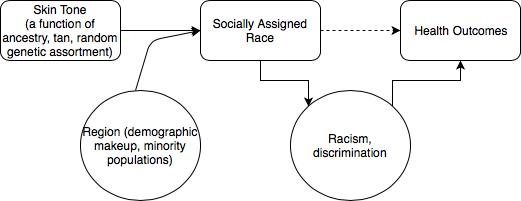
\includegraphics[scale=.5]{Colorism.png}
\caption{Proposed model for the relationship between skin tone and health outcomes}
\label{fig:colorism}
\end{figure}
The United States is experiencing a fundamental shift in racial makeup. Multiracial and racially ambiguous people make up increasingly large shares of the population, straining the systems and bureaucracies that have for generations sorted the population on the basis of race. \cite{Alba2018} These people often self-sort into the “other” category when racially stratified on hospital intake forms or when filling out the Census. \cite{Macintosh2013,Cobb2016,Jones2008} This does not, however, mean that they are without a race. Race is widely accepted in sociology to be an externally defined, socially constructed manner of sorting people.\cite{Cobb2016} With shifting racial categories whose boundaries include varying parts of the populace from Census to Census, race is occasionally as ambiguous as the people it fails to categorize. \cite{Alba2018, Morning2018}
This project seeks to lend some clarity to how this issue of racial ambiguity complicates existing racial disparities in health. To address this, I will ask how geographic context affects skin tone-based disparities in health. Specifically, I am interested in how the racial and minority makeup of a location impacts the effect of skin tone on health. I hypothesize that geography acts as a mediator on skin tone for racially ambiguous people as demonstrated in this proposed model (Figure \ref{fig:colorism}).  

This project relies on existing literature around racial differences in health, skin tone differences in health within racial groups, and local context as a factor in individual understandings of race and ethnicity. It seeks to understand how skin tone and race exist separately from each other and, in turn, how assigned race (derived from local context) leads to skin tone disparities in health. 
\section{Analysis}

% latex table generated in R 3.2.2 by xtable 1.8-4 package
% Sat Nov 30 12:22:12 2019
\begin{table}[ht]
\centering
\begin{tabular}{rrrrrrrrrrr}
  \hline
 & 1 & 2 & 3 & 4 & 5 & 6 & 7 & 8 & 9 & 10 \\ 
  \hline
New England & 281 & 119 & 20 & 10 &  8 &  6 &  3 &  4 &  0 & 12 \\ 
  Mid Atlantic & 425 & 182 & 92 & 42 & 59 & 27 & 24 & 31 & 11 &  6 \\ 
  E. Nor. Central & 745 & 455 & 137 & 55 & 32 & 31 & 32 & 16 &  8 &  1 \\ 
  W. Nor. Central & 213 & 152 & 75 & 33 & 18 & 18 & 11 &  8 &  2 &  1 \\ 
  South Atlantic & 697 & 451 & 160 & 96 & 93 & 78 & 102 & 68 & 30 & 14 \\ 
  E. Sou. Central & 226 & 131 & 55 & 37 & 44 & 23 & 30 & 20 &  5 &  0 \\ 
  W. Sou. Central & 271 & 274 & 148 & 72 & 35 & 32 & 24 & 29 & 15 &  1 \\ 
  Mountain & 272 & 250 & 91 & 37 & 23 & 16 & 16 &  8 &  3 &  0 \\ 
  Pacific & 429 & 371 & 214 & 98 & 48 & 16 & 16 & 11 &  9 &  1 \\ 
   \hline
\end{tabular}
\caption{Skin Tone Frequency by Region} 
\label{tab:table1}
\end{table}
To begin to assess the strength of this argument, I used GSS data from 2012-18. In these years, respondents’ skin tone was assessed by the interviewing, allowed for a proxy of socially assigned race. I used the nine intervals of skin tone as the independent variable and used three different measures of self-reported health as the dependent variables: days of poor mental health in the past month, days of activity limitation in the past month, and general health. I also used the GSS delineations of respondent region to categorize results by region. 

As show in Table \ref{tab:table1}, the distribution of skin tone across the country is is not constant. These regional differences serve to support initial understandings of the different skin tone/health trends
\begin{figure}[h!]
\centering
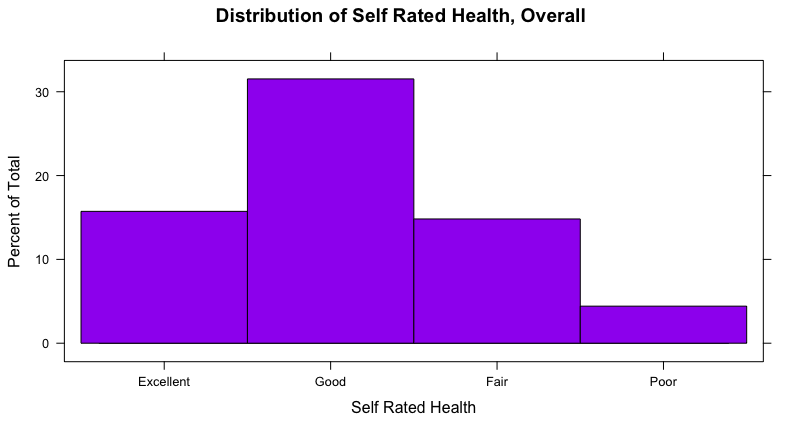
\includegraphics[scale=.3]{SelfRatedHealthOverall.png}
\caption{Self rated health overall, nationally}
\label{fig:SRHOverall}
\end{figure}
\begin{figure}[h!]
\centering
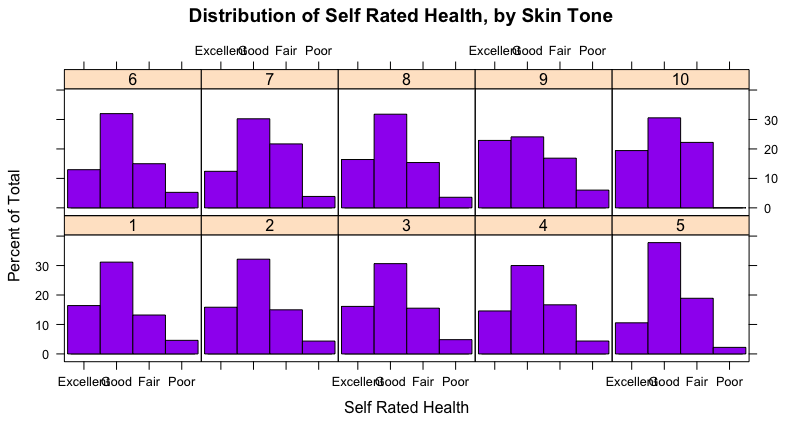
\includegraphics[scale=.3]{SelfRateHealthTone.png}
\caption{Self rated health by skin tone, nationally}
\label{fig:SRHTone}
\end{figure}
Overall, self reported health deviates from aggregate trends when stratified by skin tone. As shown in Figure \ref{fig:SRHOverall}, about 30\% of respondents reported good health. Figure \ref{fig:SRHTone} shows, however, that this patterning is not constant across skin tones. This indicates that health does vary with skin tone. 

Finally, to combine these two threads, Figure \ref{fig:activitynational} and Figure \ref{fig:activityregional} show us that while days of activity limitation increase with skin color, this relationship is not constant across region. 

\begin{figure}[H]
\centering
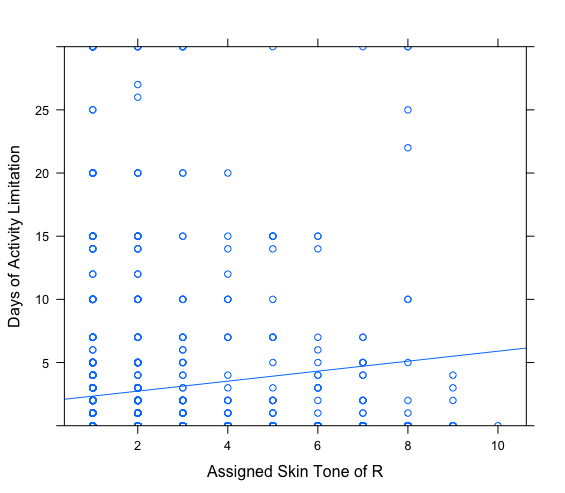
\includegraphics[scale=.3]{nationalactivitylimitation.png}
\caption{Days of activity limitation in past month due to health, nationally}
\label{fig:activitynational}
\end{figure}
\begin{figure}[H]
\centering
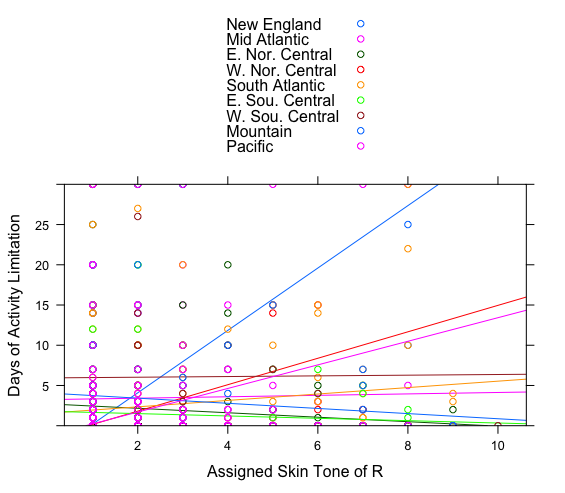
\includegraphics[scale=.3]{regionalactivity.png}
\caption{Days of activity limitation in past month due to health, by region}
\label{fig:activityregional}
\end{figure}

\section{Conclusion}
The preliminary results show that, while nationally people with darker skin experience worse health, the effect is not constant across regions. In some places, the penalties for dark skin are higher than others. These regions have different demographic compositions than those where the penalties are lower, lending credence to the idea that geographic context, at least at the regional level, matters. 

\bibliographystyle{plain}
\bibliography{Colorism}
\end{document}
